


%%%%%%%%%%%%%%%%%%%%%%%%%%%%%%%%%%%%%%%%%%%%%%%%%%%%%%%%%%%%%%%%%%%%%%%%%%
\begin{figure}[htb]
    %   \documentclass{standalone}
    %   \usepackage{pgfplots}
    %   \pgfplotsset{compat=1.18} % Kompatibilität für neuere Versionen
           \centering
           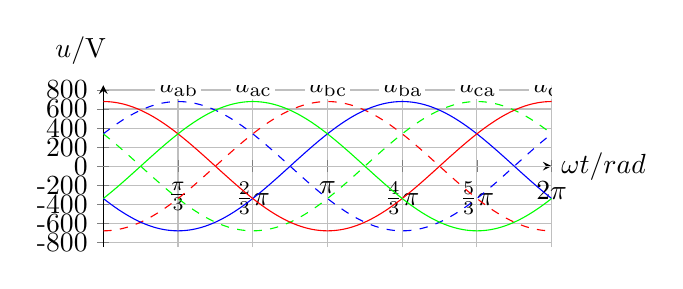
\begin{tikzpicture}
               \begin{axis}[
                   % x/y range adjustment
                   xmin=0, xmax=360,
                   ymin=-850, ymax=850,
                   samples=500,
                   axis y line=center,
                   axis x line=middle,
                   extra y ticks=0,
                   % Label text
                   xlabel={$\omega t / \text{rad}$},,
                   ylabel={$u/\mathrm{V}$},
                   % Label adjustment
                   x label style={at={(axis description cs:1,0.5)},anchor=west},
                   y label style={at={(axis description cs:-.05,.97)},anchor=south,yshift=0.2cm},
                   width=0.6\textwidth,
                   height=0.3\textwidth,
                   % x-Ticks
                   xtick={0,60,120,180,240,300,360},
                   xticklabels={,$\frac{\pi}{3}$,$\frac{2}{3}\pi$,$\pi$, $\frac{4}{3}\pi$,$\frac{5}{3}\pi$,$2\pi$},
                   xticklabel style = {anchor=north},
                   % y-Ticks
                   ytick={800,600,400,200,0,-200,-400, -600,-800},
                   yticklabels={800,600,400,200,0,-200,-400, -600,-800},
                   yticklabel style = {anchor=east},
                   % Grid layout
                   grid,
                   %grid style={line width=.1pt, draw=gray!10},
                   %major grid style={line width=.2pt,draw=gray!90},
                     ]
               % Voltage u1a(wt), u1b(wt) u1c(wt)
               \addplot[blue, domain= 0:360,dashed] {678.82*sin(x+30)};
               \addplot[red, domain= 0:360,dashed] {678.82*sin(x-90)};
               \addplot[green, domain= 0:360,dashed] {678.82*sin(x-210)};
               \addplot[blue, domain= 0:360,solid] {-678.82*sin(x+30)};
               \addplot[red, domain= 0:360,solid] {-678.82*sin(x-90)};
               \addplot[green, domain= 0:360,solid] {-678.82*sin(x-210)};
               % Label of u1c
               \node[black, fill=white, inner sep = 1pt, anchor = south] at (axis cs:180,700) {$u_{\mathrm{bc}}$}; 
               % Label of u1a
               \node[black, fill=white, inner sep = 1pt, anchor = south] at (axis cs:60,700) {$u_{\mathrm{ab}}$};           
               % Label of u1b
               \node[black, fill=white, inner sep = 1pt, anchor = south] at (axis cs:120,700) {$u_{\mathrm{ac}}$};
               % Label of u1b
               \node[black, fill=white, inner sep = 1pt, anchor = south] at (axis cs:240,700) {$u_{\mathrm{ba}}$};
               % Label of u1b
               \node[black, fill=white, inner sep = 1pt, anchor = south] at (axis cs:300,700) {$u_{\mathrm{ca}}$};
               % Label of u1b
               \node[black, fill=white, inner sep = 1pt, anchor = south] at (axis cs:360,700) {$u_{\mathrm{cb}}$};

           \end{axis}     
           \end{tikzpicture}
           \caption{Output voltage $u_\mathrm{2}(t)$ for $\alpha_\mathrm{mot}$.}
           \label{fig:Task04.2_line_voltage_B6C_with_motor_load}
   \end{figure}